\begin{figure}[h]
    \centering
    \text{Simulation of particle position for $p_0=(100, 0, 100)$,}
    \text{$v_0=(0, 1, 0)$, $\Delta t=10^{-3}$, $N=10^5$}
    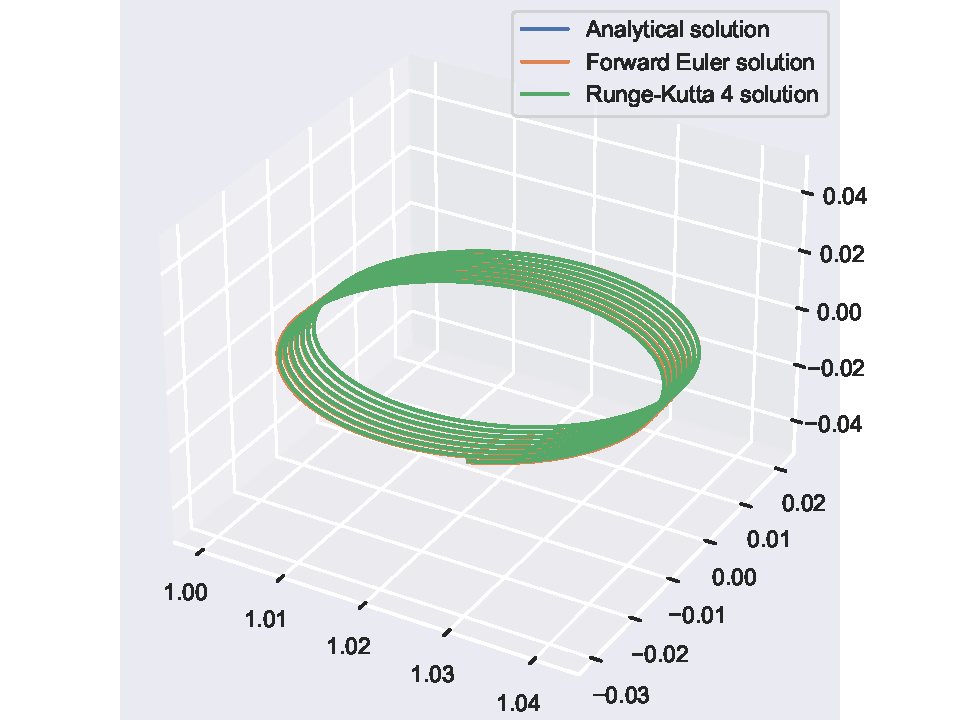
\includegraphics[width=0.5\textwidth]{data/position_estimates.pdf}
    \caption{The position of the particle as according to the analytical solution, a Forward Euler simulation and a Runge-Kutta 4 simulation}
    \label{fig:estimated_positions}
\end{figure}

Simulating the penning trap with Runge-Kutta 4 gives output that follows the analytical solution very closely. In comparison we observe some very small deviation in the solution from Forward Euler (FIG. \ref{fig:estimated_positions}). 
\\\\
Figure (\ref{fig:runge_kutta_relative_error}) more closely analyzes the error of our simulation. Here we show the relative error using 5 different step sizes and $t \in [0, 100]\mu s$. In figure (\ref{fig:forward_euler_relative_error}) we do the same for Forward Euler. Using this we get to say something about the rate of convergence for Runge-Kutta 4 and Forward Euler. For Forward Euler we estimate $r_\text{err} = 0.811$, while Runge-Kutta 4 as expected performs better at $r_\text{err} = 1.93$. While this is significantly lower than the expected $\mathcal{O}(h^4)$, this might be because this is a poor estimate. This might have something to do with the anomalies we see in figure (\ref{fig:runge_kutta_relative_error}).
\\\\
We clearly see from our results that the step size affect the precision of the simulation, with smaller step sizes giving solutions closer to the analytic one. When deciding on a step size for finding resonance, precision is obviously a concern. However smaller step sizes also gives more computationally heavy simulations. With this in mind, we decided on a step size of $h=10^{-2}$.
\\\\
It's also worth noting that the error grows as $t$ grows. This is important as we are about to look at the state of the penning trap 500$\mu s$ in.
\\\\
Figure (\ref{fig:two_particles_xy_plane}) shows the effect of turning off the coulomb interactions, as a plot of the path in the xy-plane. Figure (\ref{fig:two_particles_xy_plane_3d}) also shows the effect of turning off the interactions, with a 3D-plot of the trajectories of the particles. As expected, turning off coulomb interactions slightly alters the path of the particle. Importantly, turning off coulomb interactions greatly reduces the time it takes to carry out the simulations. This means we can simulate many more particles, as we need to when looking for resonance.
\\\\
\begin{figure}[h]
    \centering
     \text{Relative error of Runge Kutta 4}
    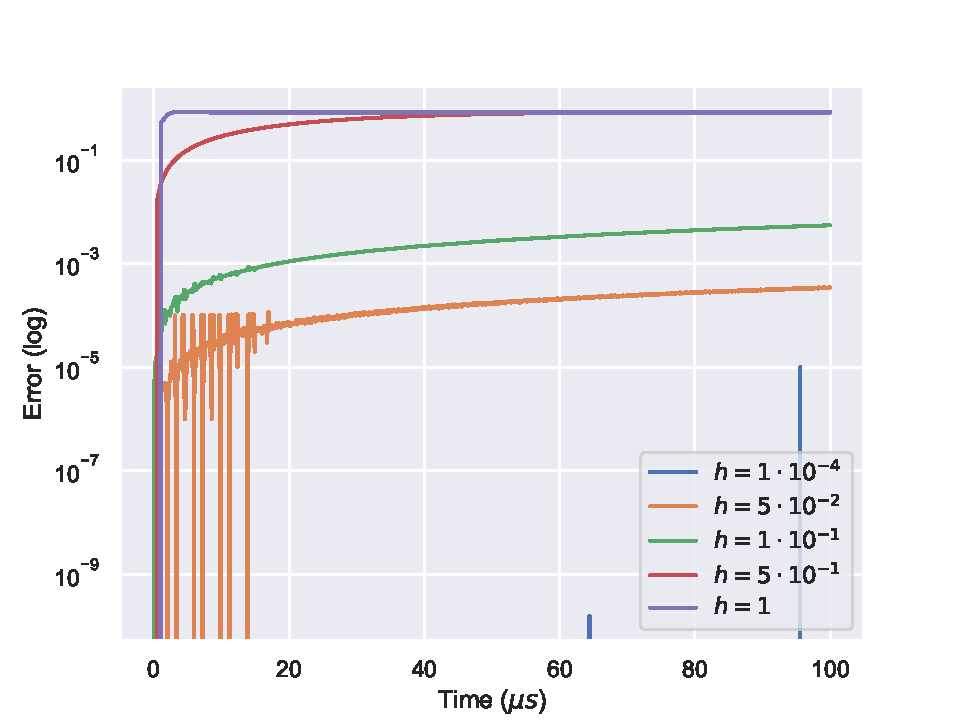
\includegraphics[width=0.5\textwidth]{data/runge_kutta_4_relativeError.pdf}
    \caption{The relative error for the Runge-Kutta 4 method as compared to the analytical solution}
    \label{fig:runge_kutta_relative_error}
\end{figure}
\begin{figure}[h]
    \centering
    \text{Relative error of Forward Euler}
    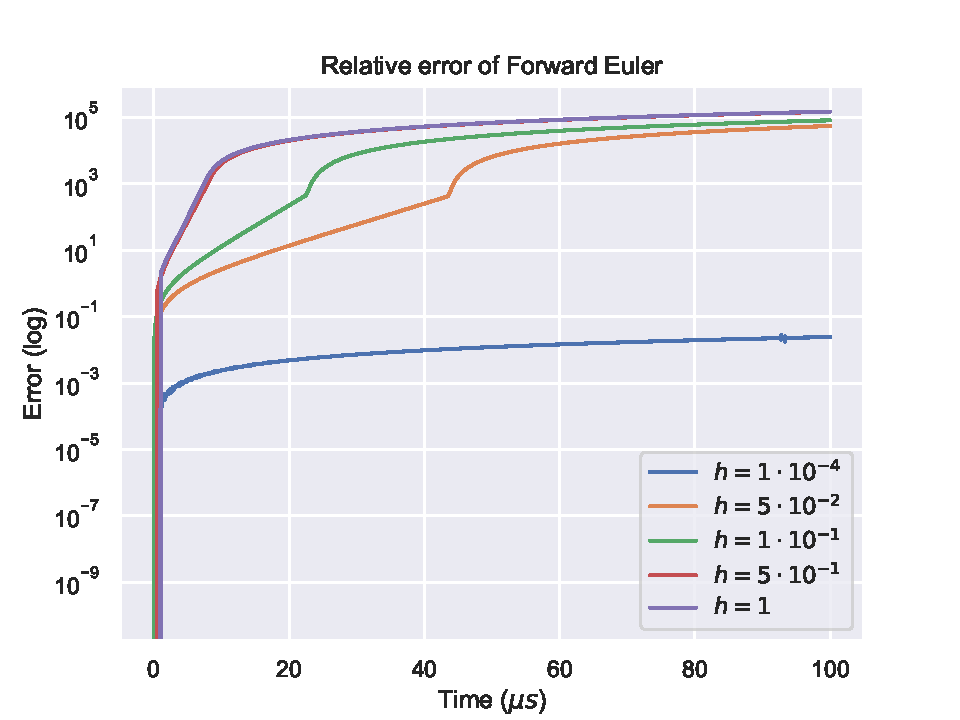
\includegraphics[width=0.5\textwidth]{data/forward_euler_relativeError.pdf}
    \caption{The relative error for the Forward Euler method as compared to the analytical solution}
    \label{fig:forward_euler_relative_error}
\end{figure}
% TODO: Place the correct place
\begin{figure}[h]
    \centering
    \text{Motion of two particles in the xy-plane}
    \text{with and without coulomb interaction}
    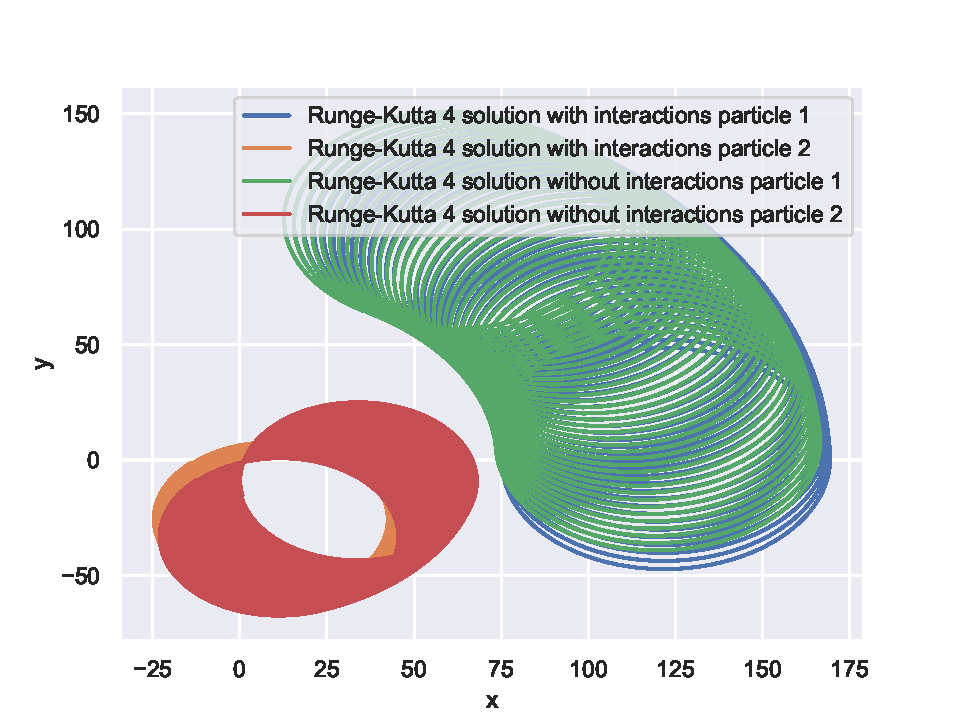
\includegraphics[width=0.5\textwidth]{data/two_particles_2d.pdf}
    \caption{The simulations of two particles with and without coulomb interactions}
    \label{fig:two_particles_xy_plane}
\end{figure}
\begin{figure}[h]
    \centering
    \text{Motion of two particles in the xy-plane}
    \text{with and without interaction in 3D}
    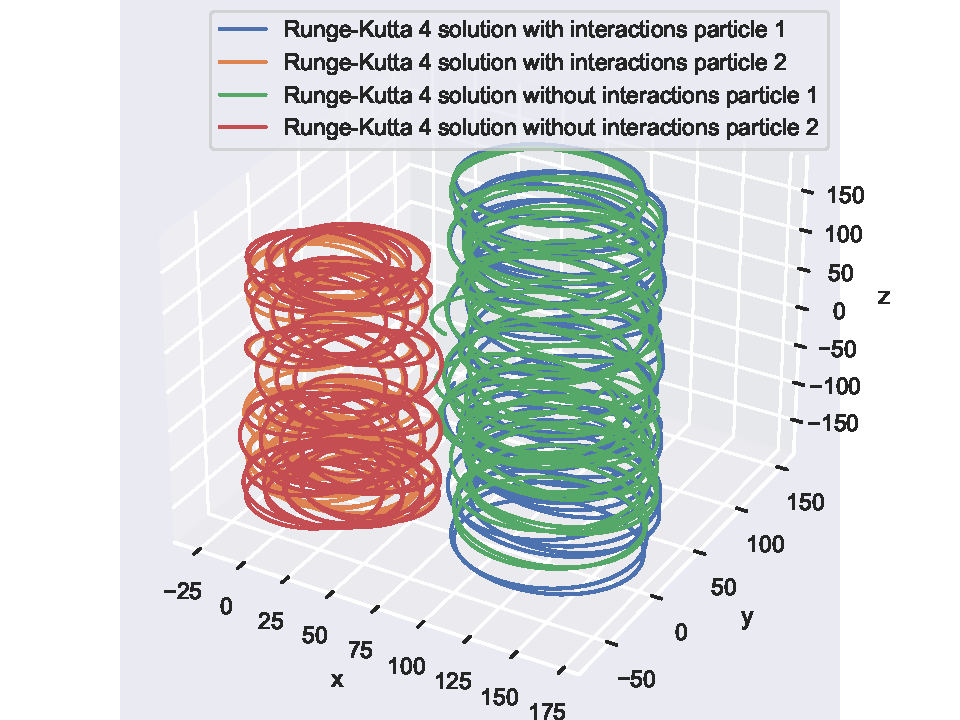
\includegraphics[width=0.5\textwidth]{data/two_particles_3d.pdf}
    \caption{The simulations of two particles with and without coulomb interactions in 3d}
    \label{fig:two_particles_xy_plane_3d}
\end{figure}

\begin{figure}[h]
    \centering
    \text{Particles left after $500$ $\mu s$}
    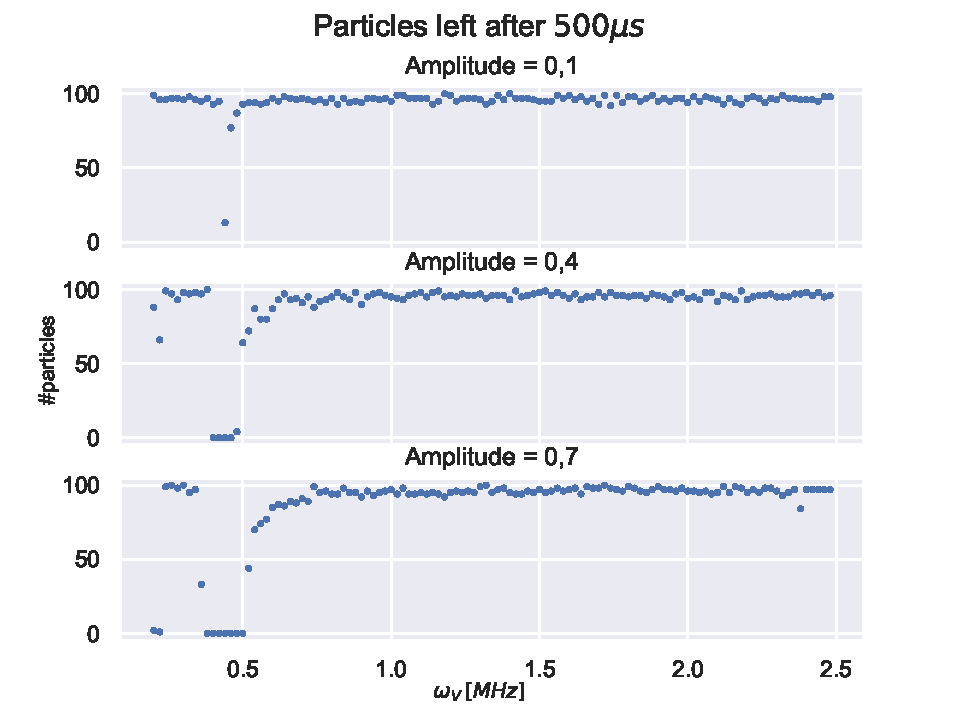
\includegraphics[width=0.5\textwidth]{data/particles_left_rough_grained.pdf}
    \caption{Particles left in the penning trap for different frequencies}
    \label{fig:particles_left_rough_grained}
\end{figure}
\begin{figure}[h]
    \centering
    \text{Particles left after $500$ $\mu s$}
    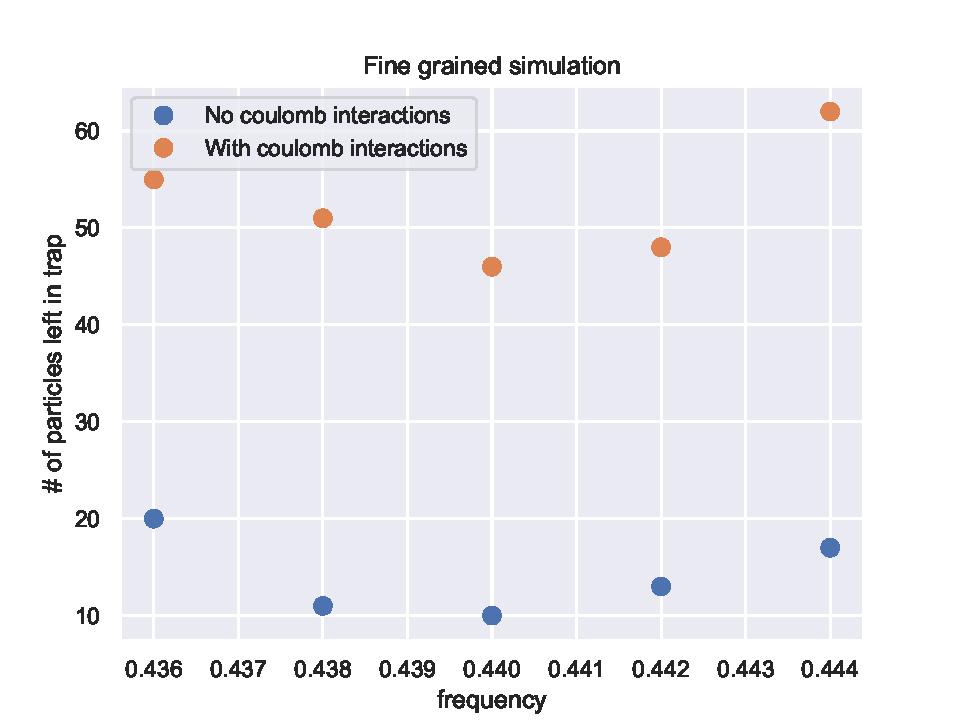
\includegraphics[width=0.5\textwidth]{data/particles_left_fine_grained.pdf}
    \caption{Particles left in the penning trap for different frequencies with and w/o coulomb interactions}
    \label{fig:particles_left_fine_grained}
\end{figure}

For a time-dependent electric field we repeated simulations of 100 $\text{Ca}^{+}$-ions with amplitudes $f = 0.1, 0.4, 0.7$, without coulomb interactions. We did the simulations for evenly spaced frequencies $\omega_V$ in the interval $[0.2, 2.5]\text{MHz}$, and counted the number of particles left in the penning trap after $500\mu s$ for a step size $h=10^{-2}$. Figure (\ref{fig:particles_left_rough_grained}) shows that for all of the amplitudes tested there is a significant lowering of the number of particles left in the trap when the frequency is $\omega_V \approx 0.44 \text{MHz}$. We also can see a clear lowering of particles left for $\omega_V \approx 0.22 \text{MHz}$ for $f=0.7$. 
\\\\
The fact that the resonance frequency at $0.22$ is half of the resonance frequency $0.44$ is a reasonable result. In general if $\omega_{V,0}$ is the fundamental frequency, the highest resonance frequency, then $\dfrac{\omega_{V,0}}{2}, \dfrac{\omega_{V,0}}{3}, \dfrac{\omega_{V,0}}{4} \ldots$ are all resonance frequencies\cite{harmonic}. In our case, $0.44$ appears to be our fundamental frequency, which fits with our finding that $\dfrac{0.44}{2}$ is also a resonance frequency.
\\\\
As the external electric force is a periodic, time-dependent force, it is natural to explain the behavior of the particles with resonance. If a calcium ion has a resonance frequency equal to the frequency $\omega_V$ of the electric field, the oscillation of the particle is amplified. This is seemingly what is happening in our simulations. If the frequency of the electric field is close to a resonance frequency of the calcium ions, the particles' oscillations increase in amplitude. This can in turn lead to the particles moving outside of the penning trap, which is why certain frequencies $\omega_V$ lead to a large amount of particles leaving the trap.
\\\\
We can also see that the breadth of the interval of frequencies where the particles all leave the trap increases as the magnitude of the electric field oscillation increases. As the magnitude increases, the oscillations become bigger.
\\\\
Next, we proceeded to do a more fine-grained simulation for $f=0.1$, both with and without coulomb interactions around $\omega_V = 0.44 \text{MHz}$. We tested with 5 evenly spaced values of $\omega_V$ in the interval $[0.436, 0.444]\text{MHz}$. As figure (\ref{fig:particles_left_fine_grained}) shows, it seems we have a local minimum for the numbers of particles left after 500$\mu s$ at around $0.44\text{MHz}$. 
\\\\
From figure (\ref{fig:particles_left_fine_grained}) it also seems we observe less resonance when accounting for the interactions between particles. This suggests that the particles' interactions disrupt the resonant oscillation that we observed without particle interactions. This result seems reasonable, as resonance occurs when a periodic force coincides with periodic movement. When coulomb interactions with 99 other particles unpredictably affects the movement of a particle, the movement is no longer perfectly periodic. Therefore it makes sense that there occurs less resonance. 
